\chapter{The Linear Paul Trap}
\label{chap:LinTrap}

\section{Single ion in a linear Paul Trap}
The linear Paul trap consists of four rods, each of which is split into three electrodes as is seen on \cref{fig:PaulTrap}. The coordinate system for the trap is defined such that the $z$-axis runs down along the centre of the trap,
while the $x,y$-axes go between diagonally opposed rods. Furthermore we define $z_0$ to be half the length of center electrodes, while we define $r_0$ as half the distance between diagoanlly opposed electrodes as seen on \cref{fig:PaulTrap}.
\begin{figure}
    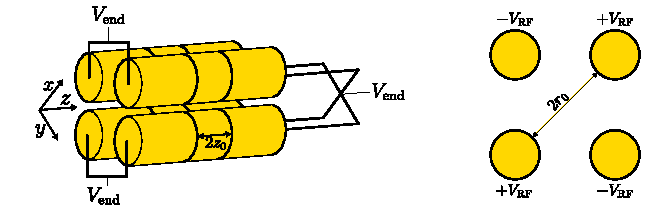
\includegraphics{main/Paul_Trap.pdf}
    \caption{Example schematic of a linear paul trap showing: (left) a 3D model of the paul Trap with both the DC endcap voltages applied.
    (right) an end-view down the Paul trap, showing the phase of the RF voltages applied to the different rods.}
    \label{fig:PaulTrap}
\end{figure}
In order to trap an ion along the $z$-direction a static voltage $V_{end}$ is applied to all of the electrodes on the end of the rods. By applying such a votlage to these endcap electrodes an electrical potential is generated, which in the region around the centre of the trap can be written as
\begin{equation}
    \phi_{DC}(z) = \frac{\kappa V_{end}}{z_0^2}z^2,
    \label{eq:phi_DC_z} 
\end{equation}
where $\kappa$ is a constant defined by the specific geometry of the trap, and $z$ is the position of the ion along the $z$ axis.
Thus an ion of mass $m$ and charge $Q$ finds itself sitting in a harmonic potential
\begin{equation}
    \label{eq:omega_z}
    V_{DC}(z) = \frac{1}{2}m\omega_z^2 z^2, \quad\omega_z = \sqrt{\frac{2Q\kappa V_{end}}{mz_0^2}},
\end{equation}
where $\omega_z$ is the frequency of the ions oscillating motion along the $z$-axis.

For the radial directions it is necessary to take a slightly different approach, indeed Earnshaw's theorem \textcolor{red}{Earnshaw} states
that it is impossible to trap a charged particle in all three directions, solely through the use of electrostatic forces. If we look at the electrical potential in the $x,y$-plane from the DC endcaps we also find
\begin{equation}
    \phi_{DC}(x,y) = -\frac{\kappa V_{end}}{2z_0^2}(x^2+y^2),
\end{equation}
which is clearly repulsing the ion from the center of the trap.

To counteract this repulsive effect, we employ an RF voltage, oscillating at frequency $\Omega_{RF}$, with an amplitude $V_{RF}$ on all four rods. Neighbouring rods have opposites phases while, dioganlly opposing rods share a phase, as seen on \cref{fig:PaulTrap}.
We can then write the total time dependant electrical potential in the $x,y$-plane as \textcolor{red}{KARIN}
\begin{equation}
    \phi(x,y,t) = -\frac{\kappa V_{end}}{2z_0^2}(x^2+y^2)-\frac{V_{RF}}{2r_0^2}(x^2-y^2)\cos{(\Omega_{RF}t)},
\end{equation}
where the first term comes from the repulsing DC potential, and the second term comes from the RF voltages applied to the rods.

The equations of motion in the radial plane can be rewritten on a more compact form by adopting the notation
\begin{equation}
    \tau = \frac{\Omega_{RF}t}{2},\quad a = -\frac{4Q\kappa V_{DC}}{mz_0^2\Omega_{RF}^2},\quad q_x = -q_y = 
    \frac{2QV_{RF}}{mr_0^2\Omega_{RF}^2},
\end{equation}
which allows for the equations of motion to be written as
\begin{equation}
    \frac{\text{d}^2\rho}{\text{d}\tau^2} + (a-2q_\rho\cos{(2\tau)})\rho,\quad \rho\in\{x,y\}
    \label{eq:Mathieu}.
\end{equation}
\Cref{eq:Mathieu} is known as the Mathieu equation \textcolor{red}{CITE}, the Mathieu equation has bounded solutions for several sets of $(a,q_\rho)$ parameters,
however, the conditions usually used in experiment state that for a given value of $q_\rho$, $a$ must be found between the two curves approximated by \textcolor{red}{CITE}
\begin{align}
    &a_0(q_\rho) \approx -\frac{1}{2}q_\rho^2 +\frac{7}{128}q_\rho^4 -\frac{29}{2304}q_\rho^6+\frac{68687}{18874368}q_\rho^8,\\
    &b_1(q_\rho) \approx 1-q_\rho-\frac{1}{8}q_\rho^2+\frac{1}{64}q_\rho^3-\frac{1}{1536}q_\rho^4-\frac{11}{36864}q_\rho^5.
\end{align}
Together these two lines form what is known as a stability diagram. Since a positive DC voltage is needed for the confinement in the axial direction, we usually confine ourselves to considering stability in the $a<0$ region. A plot of the stable region for the linear Paul trap can be see on \cref{fig:Stability1}
\begin{figure}
    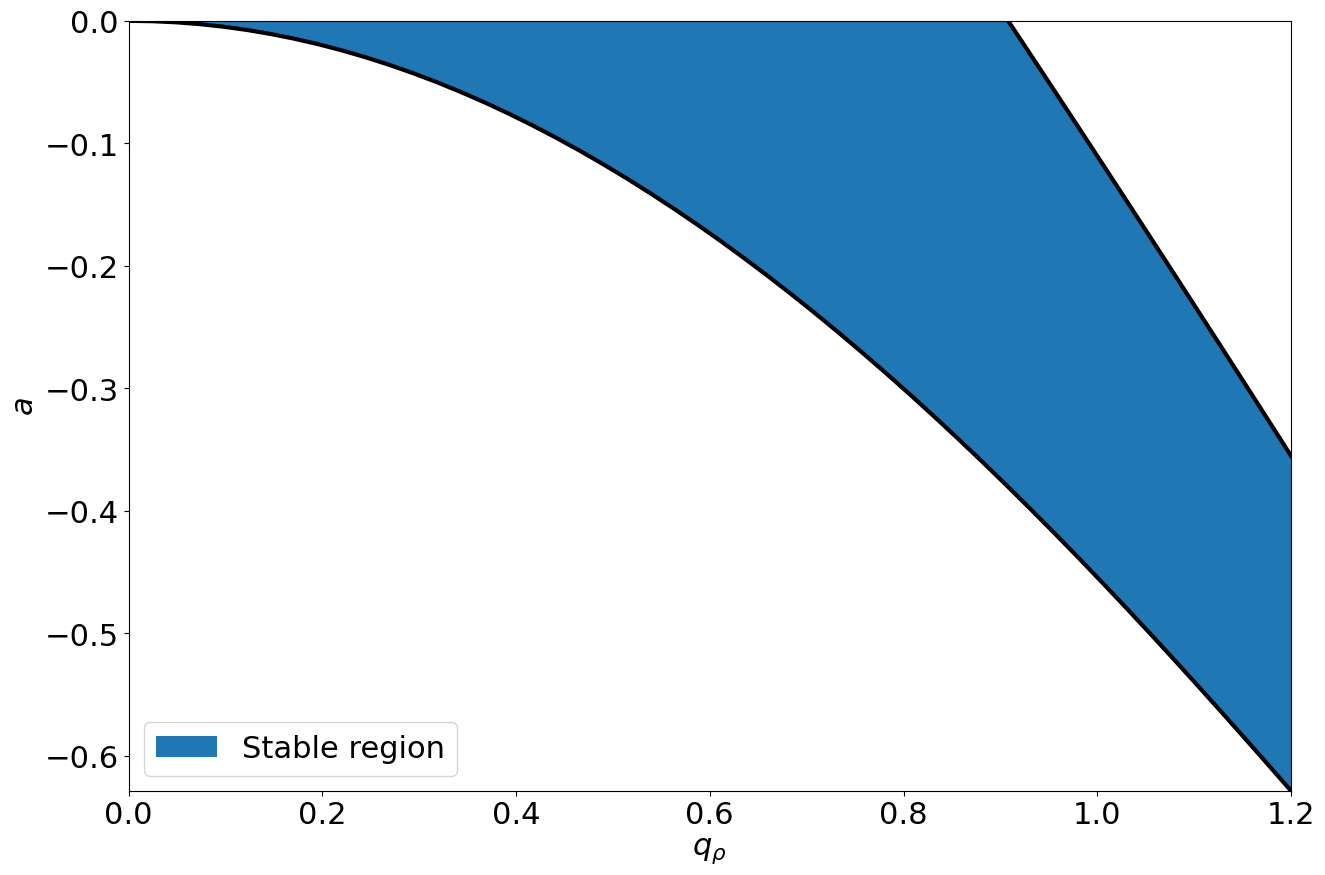
\includegraphics[width =0.8\textwidth]{main/Stability.png}
    \caption{Plot of the Mathieu stability diagram for negative values of $a$. The blue colored area contains the set of bounded, and thus stable solution to the Mathieu equation of \cref{eq:Mathieu}}
    \label{fig:Stability1}
\end{figure}

In the case where $\vert a\vert,\vert q_\rho\vert\ll 1$ the solution to \cref{eq:Mathieu} can be approximated to
\begin{equation}
    \label{eq:omega_r}
    \rho(t) = \rho_0\bigg(1-\frac{q_\rho}{2}\cos{(\Omega_{RF}t)}\bigg)\cos{(\omega_r t)},\quad \omega_r = \frac{\Omega_{RF}}{2}\sqrt{\frac{q_\rho^2}{2}+a}.
\end{equation}
Since $\vert q_\rho\vert\ll 1$ we see that there is a large-amplitude motion of the ion at frequency $\omega_r$. This motion is typically referred to as secular motion in the litterature. The frequency $\omega_r$ is much slower than the RF frequency of the trap (typically 10's-100's of kHz vs. 5MHz in the case of our trap). 

In addition there is a small-amplitude motion superimposed on top, oscillating at the RF frequency. This motion is typically referred to as micromotion. Thus the full picture we now get, is one of the ion performing slow, but large oscillations in the radial plane, with an additional micromotion on top. An example trajectory can be seen on \cref{fig:micromotion}, where the micromotion is clearly visible.



\begin{figure}
    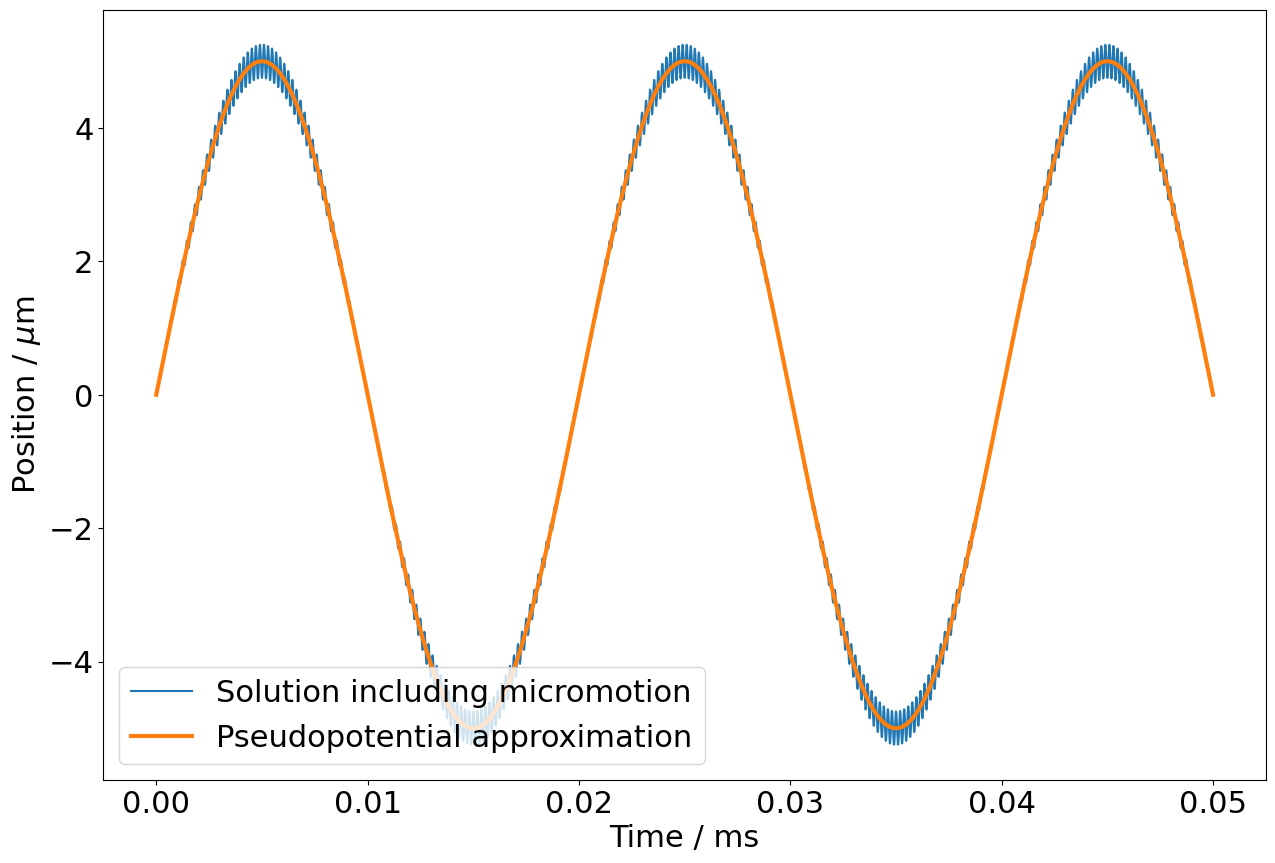
\includegraphics[width = 0.8\textwidth]{main/Micromotion.png}
    \caption{Trajectories including (blue) micromotion or calculated through the pseudopotential approximation (orange), for $\rho_0 = 5 {\mu}$m, $\omega_r = 2\pi\times 50$kHz, $\Omega_{RF} = 2\pi\times 5.2$MHz.}
    \label{fig:micromotion}
\end{figure}

It is common to average over the micromotion of the ion, keeping only the term oscillating at $\omega_r$. If this is done, it is clear that the ion then moves as if in an effective potential (often referred to as pseudopotential in the litterature) given by
\begin{equation}
    V_{Pseudo}(\rho) = \frac{1}{2}m\omega_r^2\rho^2,\quad \rho\in\{x,y\}.
\end{equation}
The pseudopotential approximation is especially useful when working with trapped ions in a quantum mechanical regime, since their Hamiltonian is then simply that of a harmonic oscillator, which is one of the most well-studied examples in all of quantum mechanics.
\section{Two ions in a linear Paul trap}
We now move on to the topic of two co-trapped ions in a Paul trap. We shall denote the ions 1 and 2 respectively, with masses $m_1,m_2$, and charges $Q_1,Q_2$.
Remembering to include the Coulomb interaction between the two ions, the potential energy of the system, in the pseudopotential approximation, can then be written as
\begin{align}
    \nonumber V(\vec{r_1},\vec{r_2}) = &\frac{1}{2}m_1\bigg(\omega_{1,z}^2z_1^2+\omega_{1,r}^2(x_1^2+y_1^2)\bigg)+\frac{1}{2}m_2\bigg(\omega_{2,z}^2+\omega_{2,r}^2(x_2^2+y_2^2)\bigg)\\
    & +\frac{Q_2Q_2}{4\pi\epsilon_0}\frac{1}{\vert r_1-r_2\vert},
\end{align}
where $\omega_{j,(r/z)}$ is calculated as in \cref{eq:omega_r,eq:omega_z}, using the mass and charge of ion $j$.
For the rest of the derivations in this report we are, unless otherwise noted, going to ignore the $y$ part of motion of the ions since our system exhibits a radial symmetry, and thus any equations that hold for $x$ will hold for $y$ as well.
